\documentclass[11pt,a4paper]{report}

\usepackage{amsmath}
\usepackage{graphicx}
\usepackage{hyperref}

\graphicspath{{images/}}

\begin{document}

\title{Part C Project Notes}
\author{Catherine Vlasov}
\maketitle

%-----------------------
\tableofcontents


%-----------------------
\chapter{Task Documentation}

All timings mentioned here are approximate. The specific results can be found in Section \ref{sec:script-timings}.

\section{Image Curation}

\subsection{Initial Image Selection}

The first step was selecting which images to use for the experiments. Flickr released a massive database of millions of images and we will use those taken by one user, referred to as \texttt{actor00003}. There are $13,349$ images taken by this user and they are on the server under \texttt{/array/vlasov/actor00003}. The largest image size in this directory is $3072\times2304$ pixels and information about all the images is in a file called \texttt{metadata.txt} in the same directory.

I wrote a script called \texttt{initial\_curation.py} to do the initial image filtering. The script uses the metadata file to identify the images that are $3072\times2304$ pixels, makes all of these images grayscale, rotates the portrait ones to landscape, and places the resulting images in a new subdirectory called \texttt{size3072}. The script took just under 20 minutes to run and 9539 grayscale, $3072\times2304$ pixel landscape images were produced.


%-----------------------
\chapter{Meeting Notes}

\section{24/10/18}

\begin{itemize}

\item What I did:
  \begin{itemize}
  \item Read Chapter 3 of the Advanced Security notes on steganography
  \item Wrote a script (\texttt{initial\_curation.py}) to find all the largest images in the \texttt{actor00003} directory and then make them all grayscale and landscape
    \begin{itemize}
    \item Wasn't quite working due to ``\texttt{Empty input file}'' error when performing multiple \texttt{jpegtran} operations
    \end{itemize}
  \end{itemize}

\item Action plan:
  \begin{enumerate}

  \item Calculate image sizes
    \begin{itemize}
    \item Preserve the 4:3 aspect ratio, not because we have to but because we can and it means we can keep things as similar as possible

    \item The largest image size we'll use is $3072\times2304$ since that's the size of the largest \texttt{actor00003} images.

    \item The smallest size will be $320\times240$ since that's a relatively common image size (and it has a 4:3 aspect ratio)

    \item The short-edge dimensions will be computed by hand by calculating $240x$ (where $x=\sqrt{1}, \sqrt{2},...,\sqrt{10}$) and then rounding to the nearest multiple of 24. Then the long-edge dimensions are calculated such that the 4:3 ratio is maintained.
    \end{itemize}

  \item Create the directory structure on the server in \texttt{/array/vlasov/}
    \begin{itemize}
    \item Keep a copy of all the original images in \texttt{actor00003/}

    \item Create one directory per image size, called \texttt{size3072} (for instance)

    \item For each size, create two subdirectories:
      \begin{enumerate}
      \item One for the unaltered images, called \texttt{cover}
      \item One per number of payload bits, called \texttt{stego-1234bits}
      \end{enumerate}

    \item Each \texttt{cover} subdirectory will have three files per cover image:
      \begin{enumerate}
      \item \texttt{image12345.jpg}: the unaltered image
      \item \texttt{image12345.costs}: the costs computed by J-UNIWARD
      \item \texttt{image12345.fea}: the features computed by JRM
      \end{enumerate}

    \item Each \texttt{stego-1234bits} subdirectory will have one file per stego image:
      \begin{enumerate}
      \item \texttt{image12345.jpg}: the stego image, which is the cover image \texttt{sizeXXXX/cover/image12345.jpg} with a 1234-bit message embedded in it
      \end{enumerate}
    \end{itemize}

  \item Crop the $3072\times2304$ cover images to the sizes calculated in task 1. Do this by cropping $8\times8$ pixel blocks evenly from the top/bottom and right/left.

  \item Generate the costs (using Dr. Ker's slighty modified J-UNIWARD code) and features (using JRM) for all the cover images of all the different sizes.
  \begin{itemize}
  \item JRM produces 22510 real numbers (the features)
  \item Up to me how to store them, but ASCII is probably the most portable
  \end{itemize}

  \item Use J-UNIWARD to embed 0.4 bits per non-zero AC coefficient in some of the covers

  \item Write a function that takes a payload size (as the number of bits) as input and computes the probabilities with which each coefficient changes during (binary) embedding.
    \begin{itemize}
    \item Goal: given the costs $c_1, c_2, ... c_N$ (where N is the total number of coefficients) of changing each coefficient (by adding/subtracting one), compute the probabilities $\pi_1, \pi_2, ..., \pi_N$ of making each of these changes

    \item Size of the payload: $\sum\limits_{i=1}^N H_2(\pi_i)$
      \begin{itemize}
      \item $H_2$ is the ``entropy'' and is defined as:
        \begin{equation*}
        H_2(x) = -x \times \log_2 x - (1-x) \times \log_2 (1-x)
        \end{equation*}

      \item Graph of $H_2$:
        \begin{center}
          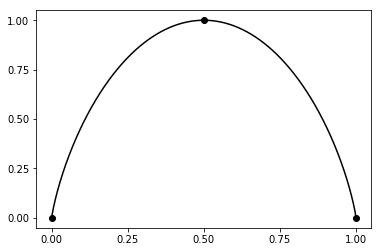
\includegraphics[width=0.7\linewidth]{h2_plot.png}
        \end{center}
      \end{itemize}

    \item Average total cost: $\sum\limits_{i=1}^N c_i \pi_i$

    \item Two (equivalent) optimization problems for computing the payload size:
      \begin{enumerate}
      \item Distortion-limited sender (DLS)
        \begin{equation*}
        \text{Maximize } \sum\limits_{i=1}^N H_2(\pi_i) \text{ such that } \sum\limits_{i=1}^N c_i \pi_i \leq C
        \end{equation*}

      \item Payload-limited sender (PLS)
        \begin{equation*}
        \text{Minimize } \sum\limits_{i=1}^N c_i \pi_i \text{ such that } \sum\limits_{i=1}^N H_2(\pi_i) \geq M
        \end{equation*}
      \end{enumerate}

    \item For some fixed $\lambda$, we can compute the probabilities:
      \begin{equation*}
      \pi_i = \frac{1}{1+e^{\lambda \cdot c_i}}
      \end{equation*}

    \item We'll use PLS, where M is the payload size.
      \begin{itemize}
      \item The optimal solution is when $\sum\limits_{i=1}^N H_2(\pi_i) = M$
      \item $\sum\limits_{i=1}^N H_2(\pi_i)$ is actually monotonically increasing, so we can find a value of $\lambda$ such that $\sum\limits_{i=1}^N H_2(\pi_i) = M$ for any M we choose. Then, we can compute the probabilities $\pi_1, \pi_2, ..., \pi_N$ using this value of $\lambda$.
      \item The end goal is to do the embedding ourselves by modifying each coefficient with these probabilities.
      \end{itemize}
    \end{itemize}

  \end{enumerate}

\item \textit{Is 80 a standard JPEG quality factor (QF)?} In the massive image database released by Flickr, the most common QFs were 100, the QF used by iPhones, and 80. So we're using 80 because that gives us a greater selection of images.

\end{itemize}


\section{17/10/18}

\begin{itemize}

\item What I did:
  \begin{itemize}
  \item Read Chapters 1 and 2 of the Advanced Security notes on steganography
  \item Read the 2008 paper ``The Square Root Law of Steganographic Capacity''
  \end{itemize}

\item Discussed questions I had about Chapter 1 (Steganography) and Chapter 2 (Steganalysis) of the Advanced Security notes and about the 2008 paper.
  \begin{itemize}

  \item \textit{What is downsampling?} Shrinking

  \item \textit{When you take a pictures on your phone, what happens?} Captures raw image, immediately compresses it as a JPEG, and discards the raw image

  \item \textit{What determines a cover's ``source''?} Primarily the camera. The camera's ISO setting, in particular, is very important. The subject of the photos don't make much of a difference.

  \item \textit{In JPEG compression, don't you lose some information when dividing the image into $8\times8$ pixel blocks?} No, the DCT is linear (i.e. 1-to-1 mapping from $8\times8$ blocks to coefficients)

  \item \textit{Is a JPEG decompressed every time you view it on a computer?} Yes

  \item \textit{When LSBR is used on RGB images, which bit(s) are changed?} Good question - it depends, but usually the LSBs of all three components (in sync)

  \end{itemize}

\item After embedding a payload, the original cover is destroyed. Otherwise, two nearly identical images would be floating around and Alice could easily be outed if someone got their hands on both versions.

\end{itemize}


\section{03/10/18}

\begin{itemize}

\item What I did: N/A

\item Discussed software to be used for embedding (J-UNIWARD), feature extraction (JRM), and detection (ensemble of linear classifiers)
  \begin{itemize}
  \item All the software is \href{http://dde.binghamton.edu/download/stego_algorithms/}{here}
  \end{itemize}

\item Server's IP: 163.1.88.150

\item Amounts of payload to embed: $O(1)$, $O(\sqrt{n})$, $O(\sqrt{n} \log n)$, $O(n)$

\item $m \sim \frac{\sqrt{DC}}{2} \log \frac{C}{D}$

\item TIME EVERYTHING

\item I will test new embedding and new detecting methods and I could also try old embedding and new detecting methods

\item Total amount of space needed (assuming around 10,000 images are used):
  \begin{itemize}
  \item Images: $2MB \times 10000 \times 9 \approx 180GB$
  \item Costs: $8B \times 5M \times 10000 \approx 400 GB$
  \item Features: $170KB \times 10000 \times 9 \approx 17GB$
  \end{itemize}

\end{itemize}


%-----------------------
\chapter{Notes to Self}

\section{Useful Commands}

\begin{itemize}

\item Run a command in the background so that you can keep using the terminal or close it
  \begin{itemize}
  \item \texttt{nohup python script.py \&> script\_output.out \&}
  \end{itemize}

\item Check on processes that are running
  \begin{itemize}
  \item \texttt{ps aux | grep vlasov}
  \end{itemize}

\end{itemize}


\section{Script Timings}
\label{sec:script-timings}

\begin{itemize}

\item \texttt{initial\_curation.py}
  \begin{itemize}
  \item $1131.18478608s \approx 18m51s$ (30/10/18)
  \end{itemize}

\end{itemize}

\section{Lessons Learned}

\begin{itemize}

\item The input and output file to \texttt{jpegtran} can't be the same, otherwise you get an ``\texttt{Empty input file}'' error.

\end{itemize}

\end{document}